\documentclass[12pt]{report}

% Packages
\usepackage{amsmath}
\usepackage{amsthm}
\usepackage{amsfonts}
\usepackage{epigraph}
\usepackage{geometry}
\usepackage{graphicx}
%\usepackage{mdframed}
\usepackage{titlesec}
\usepackage{caption}
\usepackage{listings}
\usepackage{xcolor}
\usepackage{siunitx}
\usepackage{enumitem}
\usepackage{pdfpages}
\usepackage[utf8]{inputenc}
\usepackage[hidelinks, colorlinks=true, linkcolor=blue, urlcolor=blue, citecolor=blue]{hyperref}
\usepackage[backend=biber, style=ieee]{biblatex}
\addbibresource{medical_cw.bib}

% Document Setup
\geometry{
    a4paper,
    margin=2cm,
    top=2cm,    % Adjust top margin
    bottom=2cm  % Adjust bottom margin
}

% Customise Chapter Headings
\titleformat{\chapter}
    {\normalfont\Huge\bfseries}
    {\thechapter.}
    {1em}
    {}
\titlespacing*{\chapter}{0pt}{-20pt}{\baselineskip}

% Customise section spacing
\titlespacing*{\section}{0pt}{\baselineskip}{0.5\baselineskip}

% Adjust the spacing above and below equations globally
\usepackage{etoolbox} % For \AtBeginDocument
\AtBeginDocument{
  \setlength{\abovedisplayskip}{0pt} % Space above equations
  \setlength{\belowdisplayskip}{10pt} % Space below equations
  \setlength{\abovedisplayshortskip}{0pt} % Space above when the previous line of text is short
  \setlength{\belowdisplayshortskip}{10pt} % Space below when the next line of text is short
}

% Adjusting space around figures
\setlength{\floatsep}{5pt}
\setlength{\textfloatsep}{5pt}

% Adjusting caption spacing
\captionsetup{aboveskip=5pt, belowskip=5pt}

% Format paragraphs
\setlength{\parindent}{0pt}
\setlength{\parskip}{1em}  % Adjust the value as needed

% Adjust list spacing
%\setlist[enumerate]{before=\vspace{0.5em}, after=\vspace{0.5em}}
\setlist[enumerate]{before=\vspace{-0.5\baselineskip}, after=\vspace{-0.5\baselineskip}}

% Customise question boxes
\usepackage[framemethod=TikZ]{mdframed}
\mdfsetup{
    backgroundcolor=gray!20,
    innertopmargin=10pt,
    innerbottommargin=10pt
}

% Customise explanation boxes
\newmdenv[backgroundcolor=white]{explanation}

% Setup for code listings
\lstdefinestyle{mystyle}{
    backgroundcolor=\color{gray!10},  % Change 'backcolour' to a valid color
    commentstyle=\color{blue},
    keywordstyle=\color{magenta},
    numberstyle=\fontsize{8}{12}\selectfont\color{gray},
    stringstyle=\color{green!40!black},
    basicstyle=\ttfamily\footnotesize,
    breakatwhitespace=false,
    breaklines=true,
    captionpos=b,
    keepspaces=true,
    numbers=left,
    numbersep=10pt,
    showspaces=false,
    showstringspaces=false,
    showtabs=true,
    tabsize=2,
    aboveskip=10pt,
    belowskip=10pt
}
\renewcommand{\lstlistingname}{Code Block}

% Setup for inline code
\lstdefinestyle{inline}{
    basicstyle=\ttfamily\color{black}, % Use monospaced font with default text color
    breakatwhitespace=false,
    breaklines=true,
    keepspaces=true, % Keeps spaces in text, useful for keeping indentation
    showspaces=false, % Do not show space characters
    showstringspaces=false, % Do not highlight spaces within strings
    showtabs=false, % Do not show tab characters explicitly
}
\newcommand{\inlinecode}[1]{\lstinline[style=inline]{#1}}


% Increment section number by 1 for display purposes
%\renewcommand{\thesection}{\the\numexpr\value{section}\relax}

% Use lowercase Roman numerals for subsections
%\renewcommand{\thesubsection}{\thesection.\roman{section})}

% Set the default style to your custom style
\lstset{style=mystyle}


% Word count:
% ctrl+shit+p word count

%%%%%%%%%%%%%%%%%%%%%%%%%%%%%%%%%%%%%%%%%%%%%%%%%%%%%%%%%

\begin{document}

% Title Page
\begin{titlepage}
    \centering
    
\includegraphics[width=0.3\textwidth]{crest.png}\par\vspace{1cm}
    {\Huge\bfseries Data Science in Medical Imaging\par}
    {\Huge\textit {Lent Coursework}\par}
    \vspace{1cm}
    {\Large University of Cambridge\par}
    {\Large\textit{MPhil in Data Intensive Science}\par}
    \vspace{1cm}
    {\Large William Purvis\par}
    {\small Submitted: \today\par}
    {\small Word Count: 2865\par}
\end{titlepage}

% Table of Contents
\tableofcontents

\chapter{Handing DICOM data}
\section{Introduction}

The Digital Imaging and Communications in Medicine (DICOM) standard is a framework which specifies how information in medical imaging is stored, transmitted, and exchanged. \cite{noauthor_ps31_nodate, bidgood_understanding_1997} DICOM files, identified by their .dcm file extension, are comprehensive data containers that contain both pixel values (which make up the actual image), and a rich set of metadata in the .dcm header. This metadata includes information about the patient, clinical context, and specific parameters relating to the image modality and its acquisition.

In this coursework, a dataset of DICOM files for $12$ patients from the LCTSC Lung Computed Tomography (CT) Segmentation Challenge are provided.\cite{noauthor_lctsc_nodate} The dataset offers a variable number of DICOM (.dcm) files for each patient: extending from $162$ .dcm files for patient $6$, down to $117$ .dcm files for patient $9$. Within each .dcm file, the $512 \times 512$ pixel data depicts a CT scan captured along the axial plane, offering a detailed cross-sectional view of the lungs. An example slice is shown in Figure~\ref{fig:slice_54} below, before any preprocessing is applied.

\begin{figure}[ht]
    \centering
    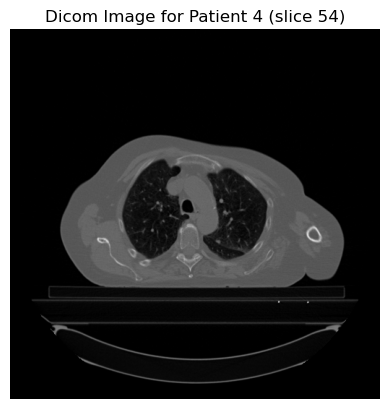
\includegraphics[width=0.4\textwidth]{slice54.png}
    \caption{Axial slice 54 for patient 4 before pre-processing}
    \label{fig:slice_54}
\end{figure}

\section{Methodology}
\label{sec:methodology}

The raw DICOM files can be processed for all patients simultaneously by running \inlinecode{python src/load_dicom.py} from the root directory of the project. The script first anonymizes the files by altering or deleting identifiable metadata tags, including \verb|PatientID|, \verb|PatientName|, \verb|PatientBirthDate|, and \verb|PatientsBirthTime|. It replaces \verb|PatientID| and \verb|PatientName| (type 2 tags, requiring a minimum of an empty string) with the case ID, clears \verb|PatientBirthDate| (setting it to an empty string), and removes the optional \verb|PatientsBirthTime| tag (type 3, allowing for deletion).
\newpage
Next, the pixel data in each .dcm file is re-scaled to \textit{Hounsfield units} (H.U.) using the \verb|RescaleSlope| and \verb|RescaleIntercept| tags and applying Equation~\ref{eq:hu}:

\begin{equation}
    \text{H.U.} = pixel value \times RescaleSlope + RescaleIntercept
    \label{eq:hu}
\end{equation}

Once the pixel data has been scaled appropriately, the \verb|SliceLocation| tag is used to order the 2D slices into a 3D NumPy array of shape [x, y, z] where x is the number of slices (axial plane), y is the coronal plane, and z is the sagittal plane.

This process is repeated for every patient (case), producing a hash map of case IDs to 3D NumPy arrays of processed DICOM data.


\section{Discussion}

In this section, a method for efficiently converting DICOM data into 3D NumPy arrays and storing these arrays in a hash map, enabling data retrieval in $O(1)$ time, was implemented. By leveraging the \texttt{SliceLocation} tag, the correct data sequence of .dcm slices was maintained regardless of directory structure or file location. This method of structuring DICOM data into a 3D array substantially improves indexing efficiency for axial (x), coronal (y), or sagittal (z) planes, facilitating both display and further analysis, as illustrated in Figure~\ref{fig:slice_54}.

\begin{figure}[ht]
    \centering
    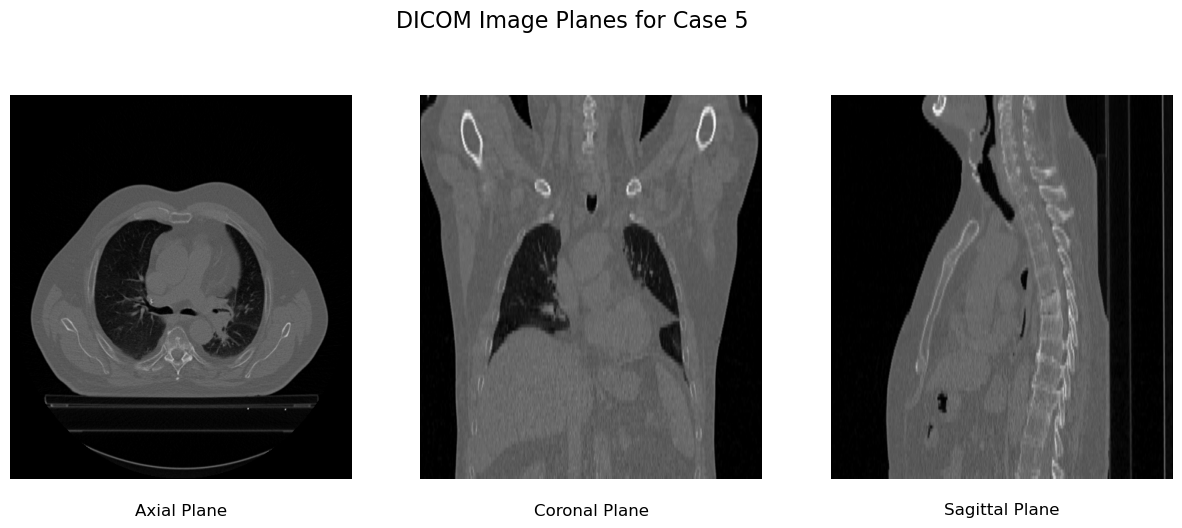
\includegraphics[width=0.8\textwidth]{planes.png}
    \caption{Slices across all three image reconstruction planes for patient 5}
    \label{fig:planes}
\end{figure}

\chapter{U-Net-based segmentation}

In addition to the DICOM files containing CT-scan data, lung segmentations for these scans are provided as NumPy arrays. These segmentations are used in the following section to train a U-Net model for image segmentation.\cite{ronneberger_u-net_2015} The U-Net architecture encompasses an encoder for downsampling, a bottleneck for feature extraction, and a decoder for upsampling, the exact architecture for the model used is shown in Figure~\ref{fig:arch}.

\begin{figure}[ht]
    \centering
    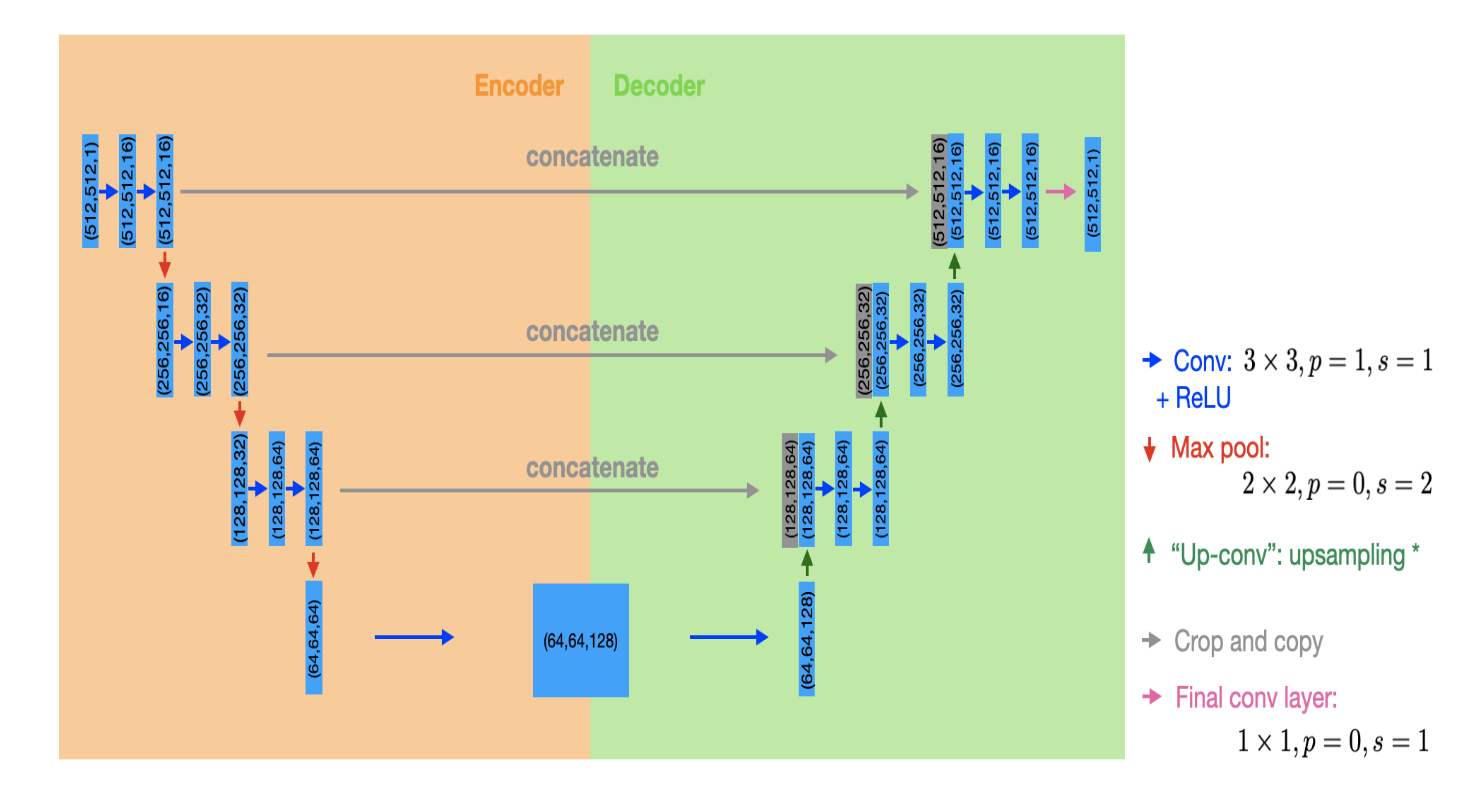
\includegraphics[width=0.8\textwidth]{unet_architecture.png}
    \caption{U-Net architecture (from practical 3)}
    \label{fig:arch}
\end{figure}
\vspace{-2em}
\section{Data preparation}

Building on the approach discussed in Section~\ref{sec:methodology}, the \inlinecode{load_patient_segmentations} function was implemented to create a hash map of case IDs to 3D NumPy arrays of segmentation data. Together with the case IDs to DICOM data dictionary, these two hash maps were combined in a custom data class (\inlinecode{DICOMSliceDataset}) for easier integration with PyTorch's data handling ecosystem, particularly the \inlinecode{DataLoader} class used for training and evaluating the U-Net model. Finally, the entire dataset was split into a training set (cases 0 to 7, with a total of 1151 2D slices) and a testing set (cases 8 to 11, with a total of 534 2D slices). The code for this data preparation is shown the Code Block~\ref{lst:split_dataset}.

\begin{lstlisting}[language=Python, caption=Splitting dataset into training and testing datasets, label=lst:split_dataset]
    # Split the data into training and validation sets (split_ratio = 0.67)
    num_train = int(len(data_dict) * split_ratio)
    num_test = len(data_dict) - num_train

    train_ids = list(data_dict.keys())[:num_train]
    test_ids = list(data_dict.keys())[num_train:]

    train_data_dict = {k: data_dict[k] for k in train_ids}
    test_data_dict = {k: data_dict[k] for k in test_ids}

    train_segmentation_dict = {k: segmentation_dict[k] for k in train_ids}
    test_segmentation_dict = {k: segmentation_dict[k] for k in test_ids}

    # Initialise the datasets
    train_dataset = DICOMSliceDataset(train_data_dict, train_segmentation_dict)
    test_dataset = DICOMSliceDataset(test_data_dict, test_segmentation_dict)
\end{lstlisting}

\section{Model training}

In order to train the U-Net model, a custom \inlinecode{ModelTrainer} class was implemented. For each training epoch, it performs a forward pass, calculates the loss, executes a backward pass to compute gradients, and updates the model parameters. It also calculates the average loss and accuracy for the epoch on both the training dataset and the test dataset. The accuracy of the model is determined using \inlinecode{BinaryAccuracy} from \inlinecode{torchmetrics.classification}:

\begin{equation}
    \text{Accuracy} = \frac{1}{N}\sum_i^N 1(y_i = \hat{y}_i)
    \label{eq:accuracy}
\end{equation}

where $y$ is a tensor of target values, and $\hat{y}$ is a tensor of predictions.

\subsection{Custom loss function}

Initially, the loss function was chosen to be \inlinecode{nn.BCELogitsLoss}, which combines a sigmoid layer and a \inlinecode{BCELoss} in a single class. This loss function is defined by Equation~\ref{eq:bceloss}.

\begin{equation}
    \text{BCELoss} = -\frac{1}{N}\sum_{i=1}^{N} y_{i}\log(\hat{y_{i}}) + (1-y_{i})\log(1-\hat{y_{i}})
    \label{eq:bceloss}
\end{equation}

After training the U-Net model for 10 epochs with a batch size of 3 and a learning rate of 0.1 using the ADAM optimiser,\cite{kingma_adam_2017} the average loss and average accuracy per epoch are shown in Figure~\ref{fig:bce_loss}.

\begin{figure}[ht]
    \centering
    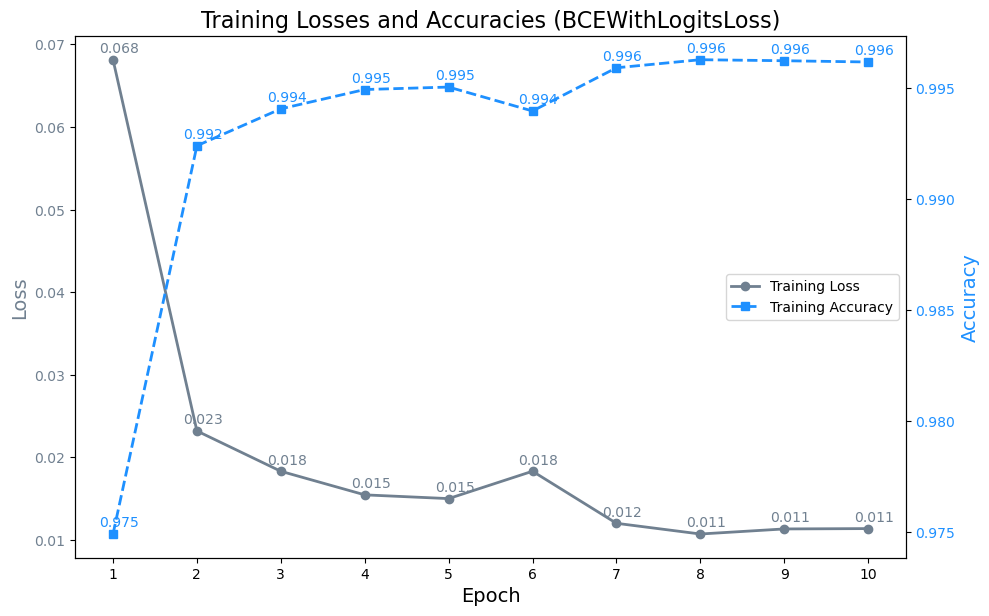
\includegraphics[width=0.8\textwidth]{bceloss.png}
    \caption{Loss and accuracy per epoch using \inlinecode{nn.BCELogitsLoss} (training dataset)}
    \label{fig:bce_loss}
\end{figure}

Next, a custom loss function was defined (in \inlinecode{src/custom_loss.py}) by combining a binary cross entropy loss with a soft Dice loss. The dice similarity coefficient (DSC) is a spatial overlap index that measures the similarity between two binary images. This measure ranges from 0 to 1, where 0 indicates no spatial overlap and 1 indicates perfect spatial overlap. The DSC is defined as:

\begin{equation}
    \text{DSC} = \frac{2\left | A\cap B \right |}{\left | A \right | + \left |  B \right |}
    \label{eq:DSC}
\end{equation}

where $\left | A\cap B \right |$ represents the common elements between sets (images) A and B, and $\left | A \right |$ and $\left | B \right |$ represent the number of elements in sets $A$ and $B$, respectively. $\left | A\cap B \right |$ can be approximated by the sum of the element-wise product of the two binary images (prediction and target mask). $\left | A \right |$ and $\left | B \right |$ can either be quantified by the sum of the elements in the binary images or by the square of the sum of the elements in the binary images.\cite{zou_statistical_2004}

In order to formulate a loss function which can be minimised, the DSC can be subtracted from unity. This is known as the \textit{soft Dice loss}:

\begin{equation}
    \text{SoftDiceLoss} = 1 - \frac{2 (\sum_{i=1}^{N} y_{i}\hat{y_{i}})+\epsilon}{\sum_{i=1}^{N} y_{i}^{2}\sum_{i}^{N} \hat{y_{i}}^{2} + \epsilon}
    \label{eq:soft_dice_loss}
\end{equation}

where $\epsilon$ is a small constant to avoid division by zero.\cite{noauthor_optimizing_nodate} 

The custom loss function combines Equations~\ref{eq:soft_dice_loss} and~\ref{eq:bceloss} to give:

\begin{equation}
    \text{CombinedLoss} = \alpha \times \text{BCELoss} + (1 - \alpha) \times \text{SoftDiceLoss}
    \label{eq:combined_loss}
\end{equation}

where $\alpha$ controls how much of each loss is combined and was set to 0.5 for this project. The average loss using the combined loss defined in Equation~\ref{eq:combined_loss} and average accuracy per epoch are shown in Figure~\ref{fig:combined_loss}.

\begin{figure}[ht]
    \centering
    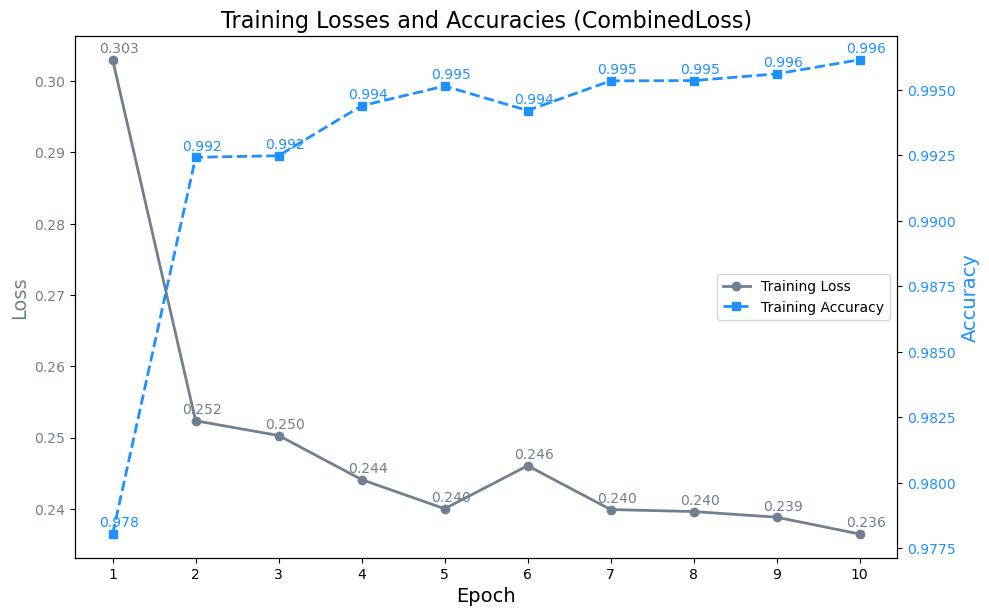
\includegraphics[width=0.8\textwidth]{combinedloss.png}
    \caption{Loss and accuracy per epoch using a custom loss function (training dataset)}
    \label{fig:combined_loss}
\end{figure}

When comparing the loss curves for the combined loss and \inlinecode{nn.BCELogitsLoss} across epochs on the training dataset, both exhibit a similar downward trend as the number of epochs increases, with the notable exception of an unexpected increase in average loss observed during epoch 6. This peak in the loss curve could be due to a batch of atypical data being used in this epoch or due to the dropout layer in the \inlinecode{maxpool_block} of the U-Net model leading to an unexpected increase in the loss. The final loss observed using the combined loss on the training set is roughly 20 times greater ($0.236$) than the final loss observed using \inlinecode{nn.BCELogitsLoss} ($0.011$). Interestingly, the accuracy curves using both loss functions are the same on the training set. The \inlinecode{nn.BCELogitsLoss} focuses on penalizing incorrect binary classifications at the pixel level without directly considering the spatial relationship between pixels. In contrast, the soft Dice Loss component in the combined loss function encourages the model to improve the overlap between predicted and ground truth segments, which inherently values the spatial coherence of the predictions. It would therefore be expected that the combined loss results in higher accuracies. As this is not the case for the training dataset, these results suggest that both loss functions may be equally effective at optimising for pixel-wise accuracy, but this does not reflect on their effectiveness at capturing the quality of the segmented regions. An extension of this work would be to vary the $\alpha$ parameter to determine what proportion of \inlinecode{SoftDiceLoss} is required to increase the accuracy during training.

The average loss and binary accuracy per epoch using both losses on the testing dataset are shown in Figures~\ref{fig:bce_loss_test} and~\ref{fig:combined_loss_test}. Both curves display anomalous behaviour with peaks in the loss function at specific epochs (epochs 2 and 6 for the combined loss, and epoch 4 for the \inlinecode{nn.BCELogitsLoss}) and mirror the trend observed across the training dataset: the final average loss is higher for the combined loss when compared to \inlinecode{nn.BCELogitsLoss}.

Both loss curves on the testing dataset exhibits unexpected fluctuations, with distinct peaks in the loss function at specific epochs: epochs 2 and 6 for the combined loss, and epoch 4 for \inlinecode{nn.BCELogitsLoss}. The overall trend echoes the trend observed in the training dataset; where the final average loss for the combined loss exceeds that of \inlinecode{nn.BCELogitsLoss} ($0.279$ versus $0.036$). This higher loss value observed with the combined loss does not necessarily indicate inferior model performance. Instead, it highlights the additional challenge posed by incorporating the \inlinecode{SoftDiceLoss} component, which demands better overlap between the predicted and true segments, not just correct individual pixel classifications. Additionally, for both loss curves, an upward trend in the loss curve is observed towards the end of training. This is indicative of overfitting: suggesting that the model does not generalise well to foreign data after epoch 8 for \inlinecode{nn.BCELogitsLoss} or after epoch 9 for the combined loss.

The higher binary accuracy observed in the model trained with the combined loss can be attributed to the fact that this model is being optimised for both pixel-wise accuracy (via \inlinecode{BCELoss}) and segmentation quality (via \inlinecode{SoftDiceLoss}). This dual optimisation helps the model to not only predict the correct pixel values, but also to do so in a way that accurately reflects the shapes and boundaries of the target segments.

\begin{figure}[ht]
    \centering
    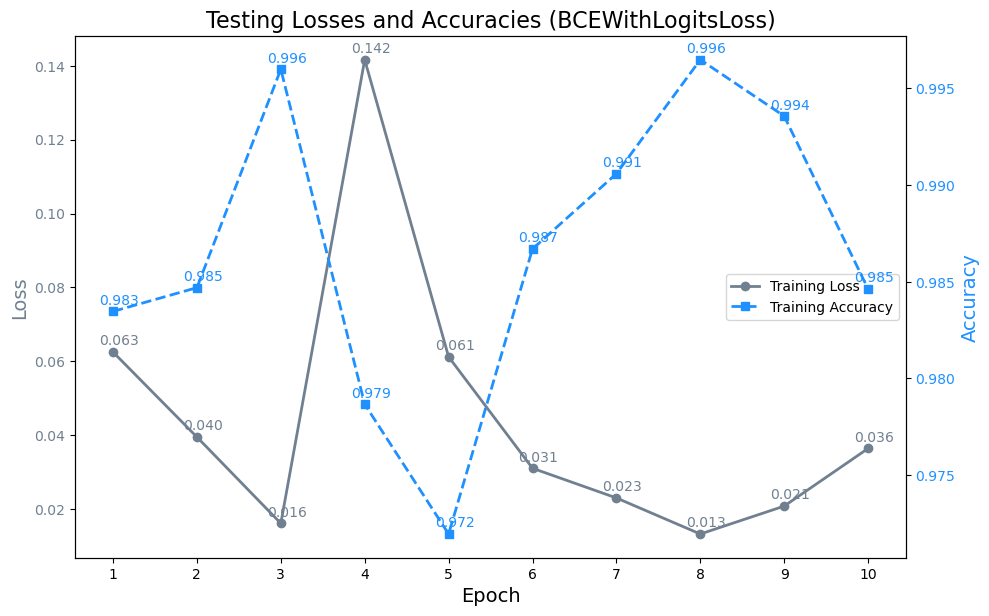
\includegraphics[width=0.8\textwidth]{bceloss_test.png}
    \caption{Loss and accuracy per epoch using \inlinecode{nn.BCELogitsLoss} (testing dataset)}
    \label{fig:bce_loss_test}
\end{figure}

\begin{figure}[ht!]
    \centering
    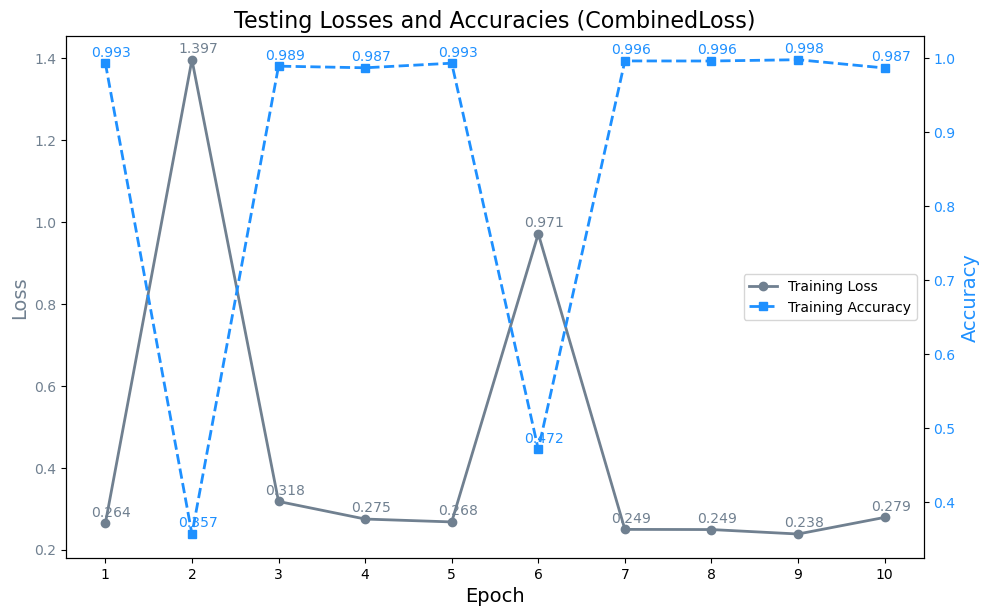
\includegraphics[width=0.8\textwidth]{combinedloss_test.png}
    \caption{Loss and accuracy per epoch using a custom loss function (testing dataset)}
    \label{fig:combined_loss_test}
\end{figure}

\section{Model evaluation}

To evaluate the U-Net model's performance with the custom loss function defined in Equation~\ref{eq:combined_loss}, the \inlinecode{evaluate_slices} method was introduced. This method calculates both binary accuracy and the Dice Similarity Coefficient (DSC), as described in Equations~\ref{eq:accuracy} and~\ref{eq:DSC}, respectively, for each 2D slice of a given dataset. It uses these metrics to compare the predicted segmentations against the ground-truth segmentations provided.

The Dice scores and binary accuracies per 2D slice in the training set are shown in Figure~\ref{fig:training_scores}. In the training set, the calculated accuracies are consistently high, fluctuating between $0.9999$ and $0.9668$. This range suggests that the model successfully learns to predict segmentations at the pixel level: accurately classifying most pixels as belonging to the target (lungs) or background. However, there is no discernable trend for the Dice scores within the training set, with values spanning from 0 to 1. This variability suggests that while the model succeeds in learning pixel-wise accuracy, it struggles to accurately delineate the overall shapes and boundaries of the segmented regions. A final explanation for the variability in Dice scores stems from the way in which the training data is loaded: to avoid learning sequence-dependent patterns and reduce overfitting, the custom \inlinecode{DICOMSliceDataset} dataclass automatically shuffles the training data. This shuffling of the data could result in the loss of any clear trend in Dice scores across 2D slices for the training set.

\begin{figure}[ht]
    \centering
    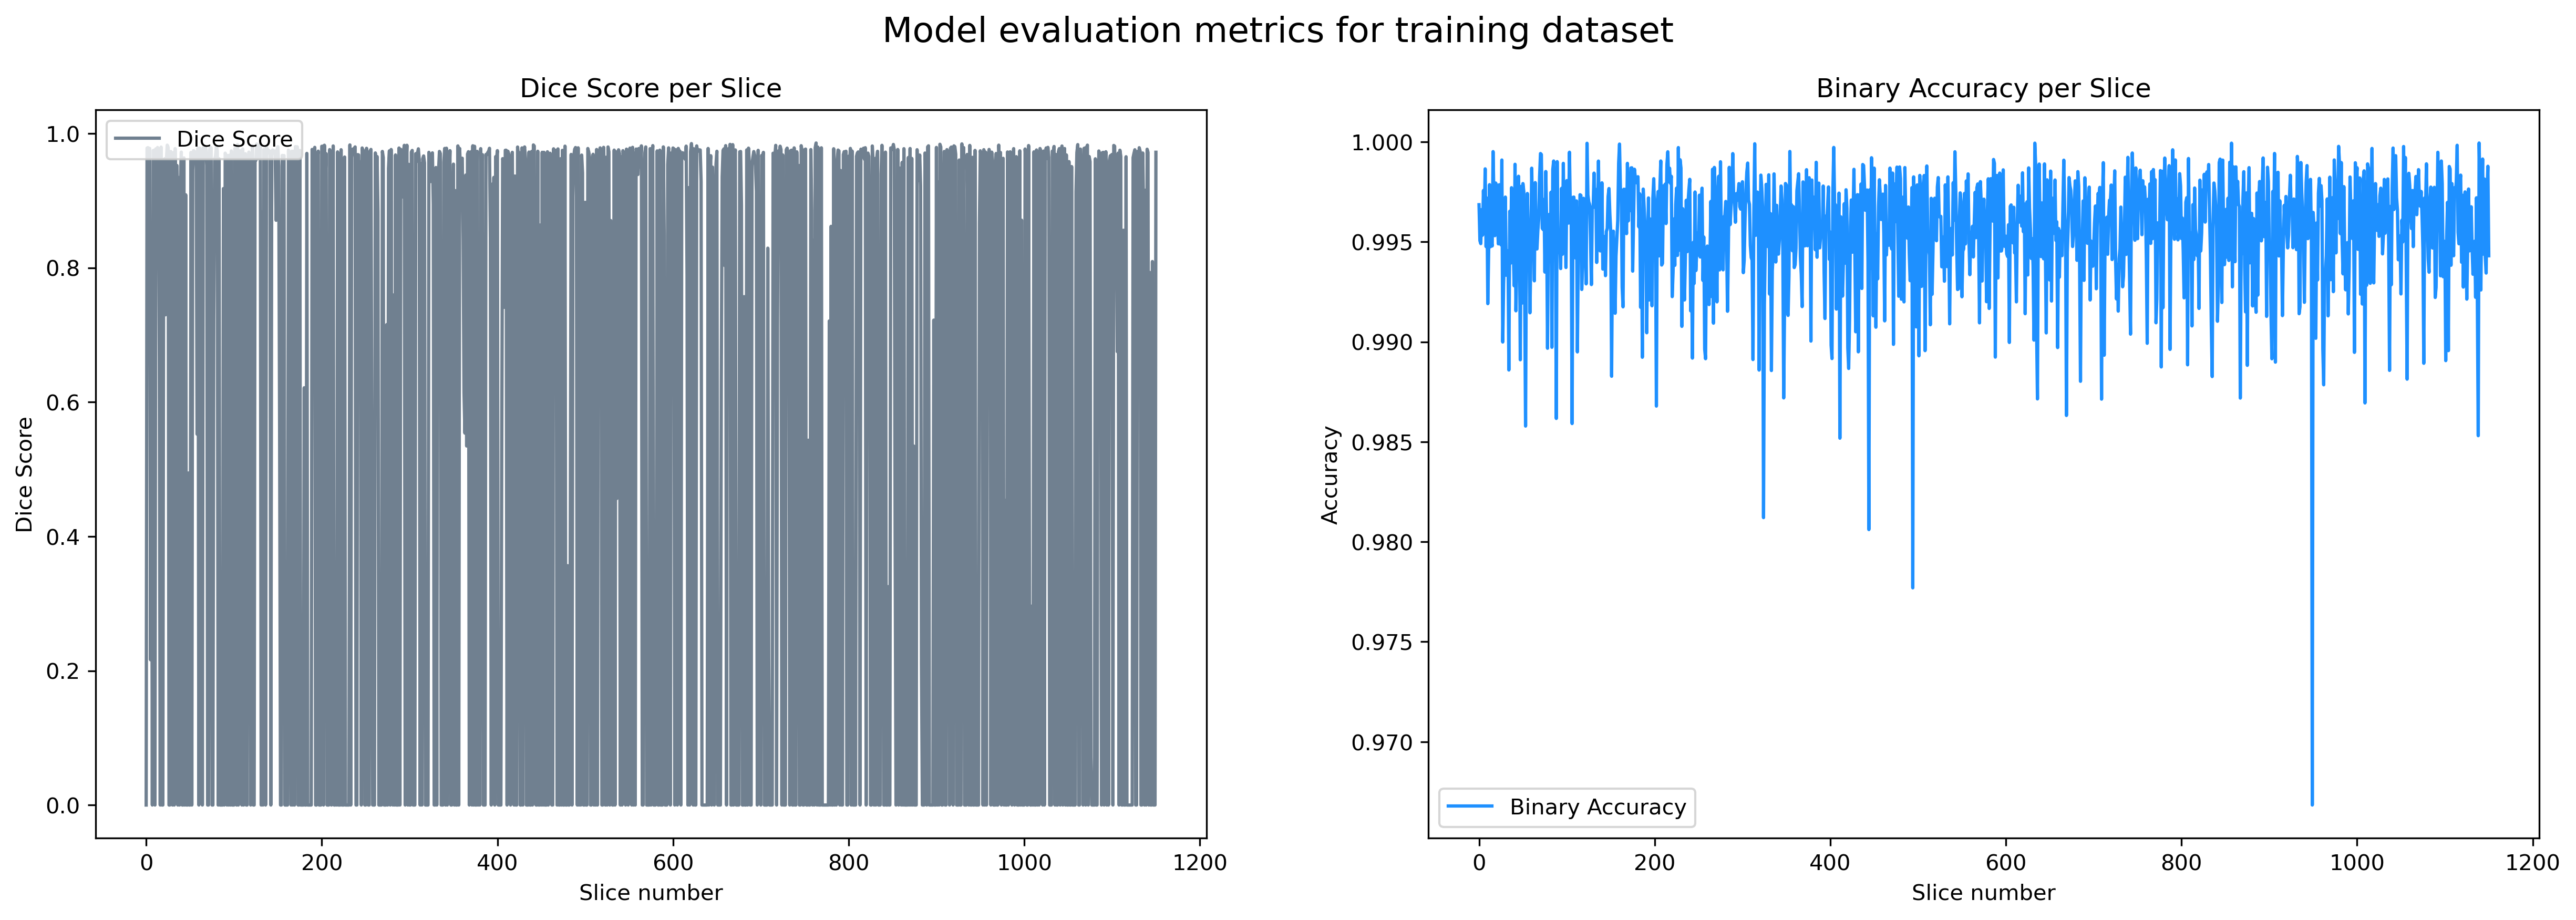
\includegraphics[width=\textwidth]{training_scores.png}
    \caption{Dice scores and binary accuracies calculated for every 2D slice in the training set}
    \label{fig:training_scores}
\end{figure}

Next, the \inlinecode{evaluate_slices} method was applied to the testing dataset, with results shown in Figure~\ref{fig:testing_scores}. This dataset, which consists of cases 8 to 11 (534 2D slices in total), exhibits a pronounced trend in Dice scores: specifically, there are four distinct peaks, each aligning with the four cases within the testing set. As the model aims to learn lung segmentations, and given that the axial planes are sequentially organised based on their \texttt{SliceLocation} tag, the instances of Dice scores equalling zero can be attributed to scans captured either before the lungs come into view, or after they have passed out of axial view. Conversely, Dice scores approaching unity are indicative of scans that effectively capture lung segmentations.

\begin{figure}[ht]
    \centering
    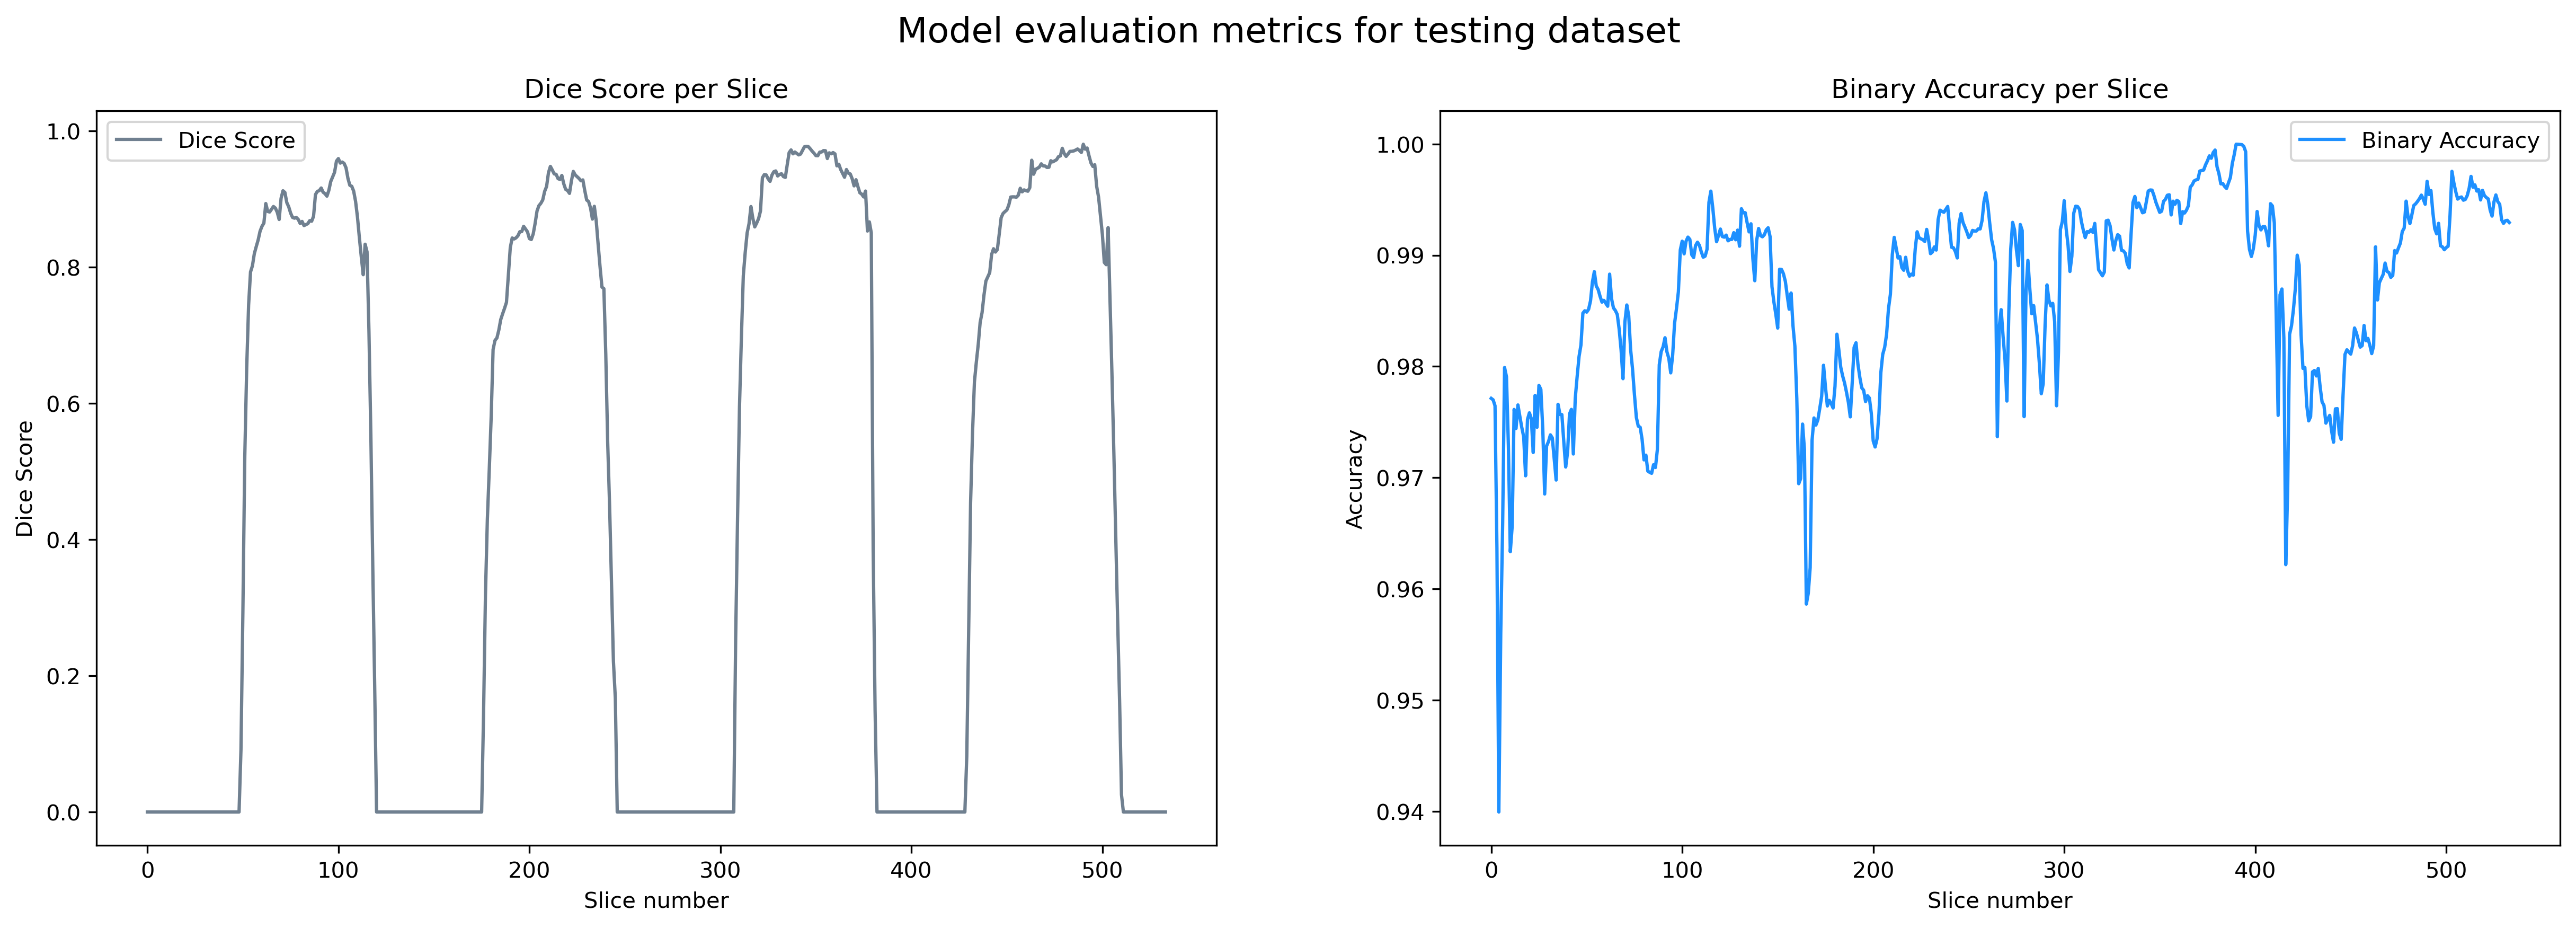
\includegraphics[width=\textwidth]{testing_scores.png}
    \caption{Dice scores and binary accuracies calculated for every 2D slice in the testing set}
    \label{fig:testing_scores}
\end{figure}

Contrary to the approach for the training set, the custom \inlinecode{DICOMSliceDataset} dataclass does not shuffle the testing data. This further implies that the lack of any clear trend in Dice scores across 2D slices in the training set is attributable to the shuffling of the training data. In the absence of shuffling, a pattern similar to that observed in the Dice scores depicted in Figure~\ref{fig:testing_scores} for the testing set would be expected, with 8 distinct peaks corresponding to the 8 cases within the training set. However, shuffling the training data remains a critical component of effective model training as it safeguards against overfitting by preventing the model from learning patterns based on the sequence of the data introduced.

The accuracies recorded for each 2D slice in the testing set remain consistently elevated, exhibiting marginally greater variance compared to those observed in the training set. Contrary to the Dice scores, the accuracies across the 2D slices for the testing data do not follow a discernible pattern, implying that the model exhibits superior generalization to unseen data in terms of delineating the overall shapes and boundaries of images—as quantified by the Dice score—rather than achieving pixel-level accuracy.

\subsection{DSC values per slice}
\label{subsec:dscs}

To highlight the performance of the trained U-Net model, three sets of plots that provide a comprehensive visualization of its effectiveness on axial slices are presented. These plots include the original CT scan image, the ground truth segmentation, and segmentations predicted by the model. Figure~\ref{fig:best_dsc_scores} shows the 2D slices that achieved the highest Dice scores, illustrating cases where the model’s predictions were very accurate, whereas, Figure~\ref{fig:worst_dsc_scores} displays the slices that recorded the lowest Dice scores. Finally, Figure~\ref{fig:med_dsc_scores} features slices that obtained median Dice scores within the testing dataset.

\begin{figure}[ht!]
    \centering
    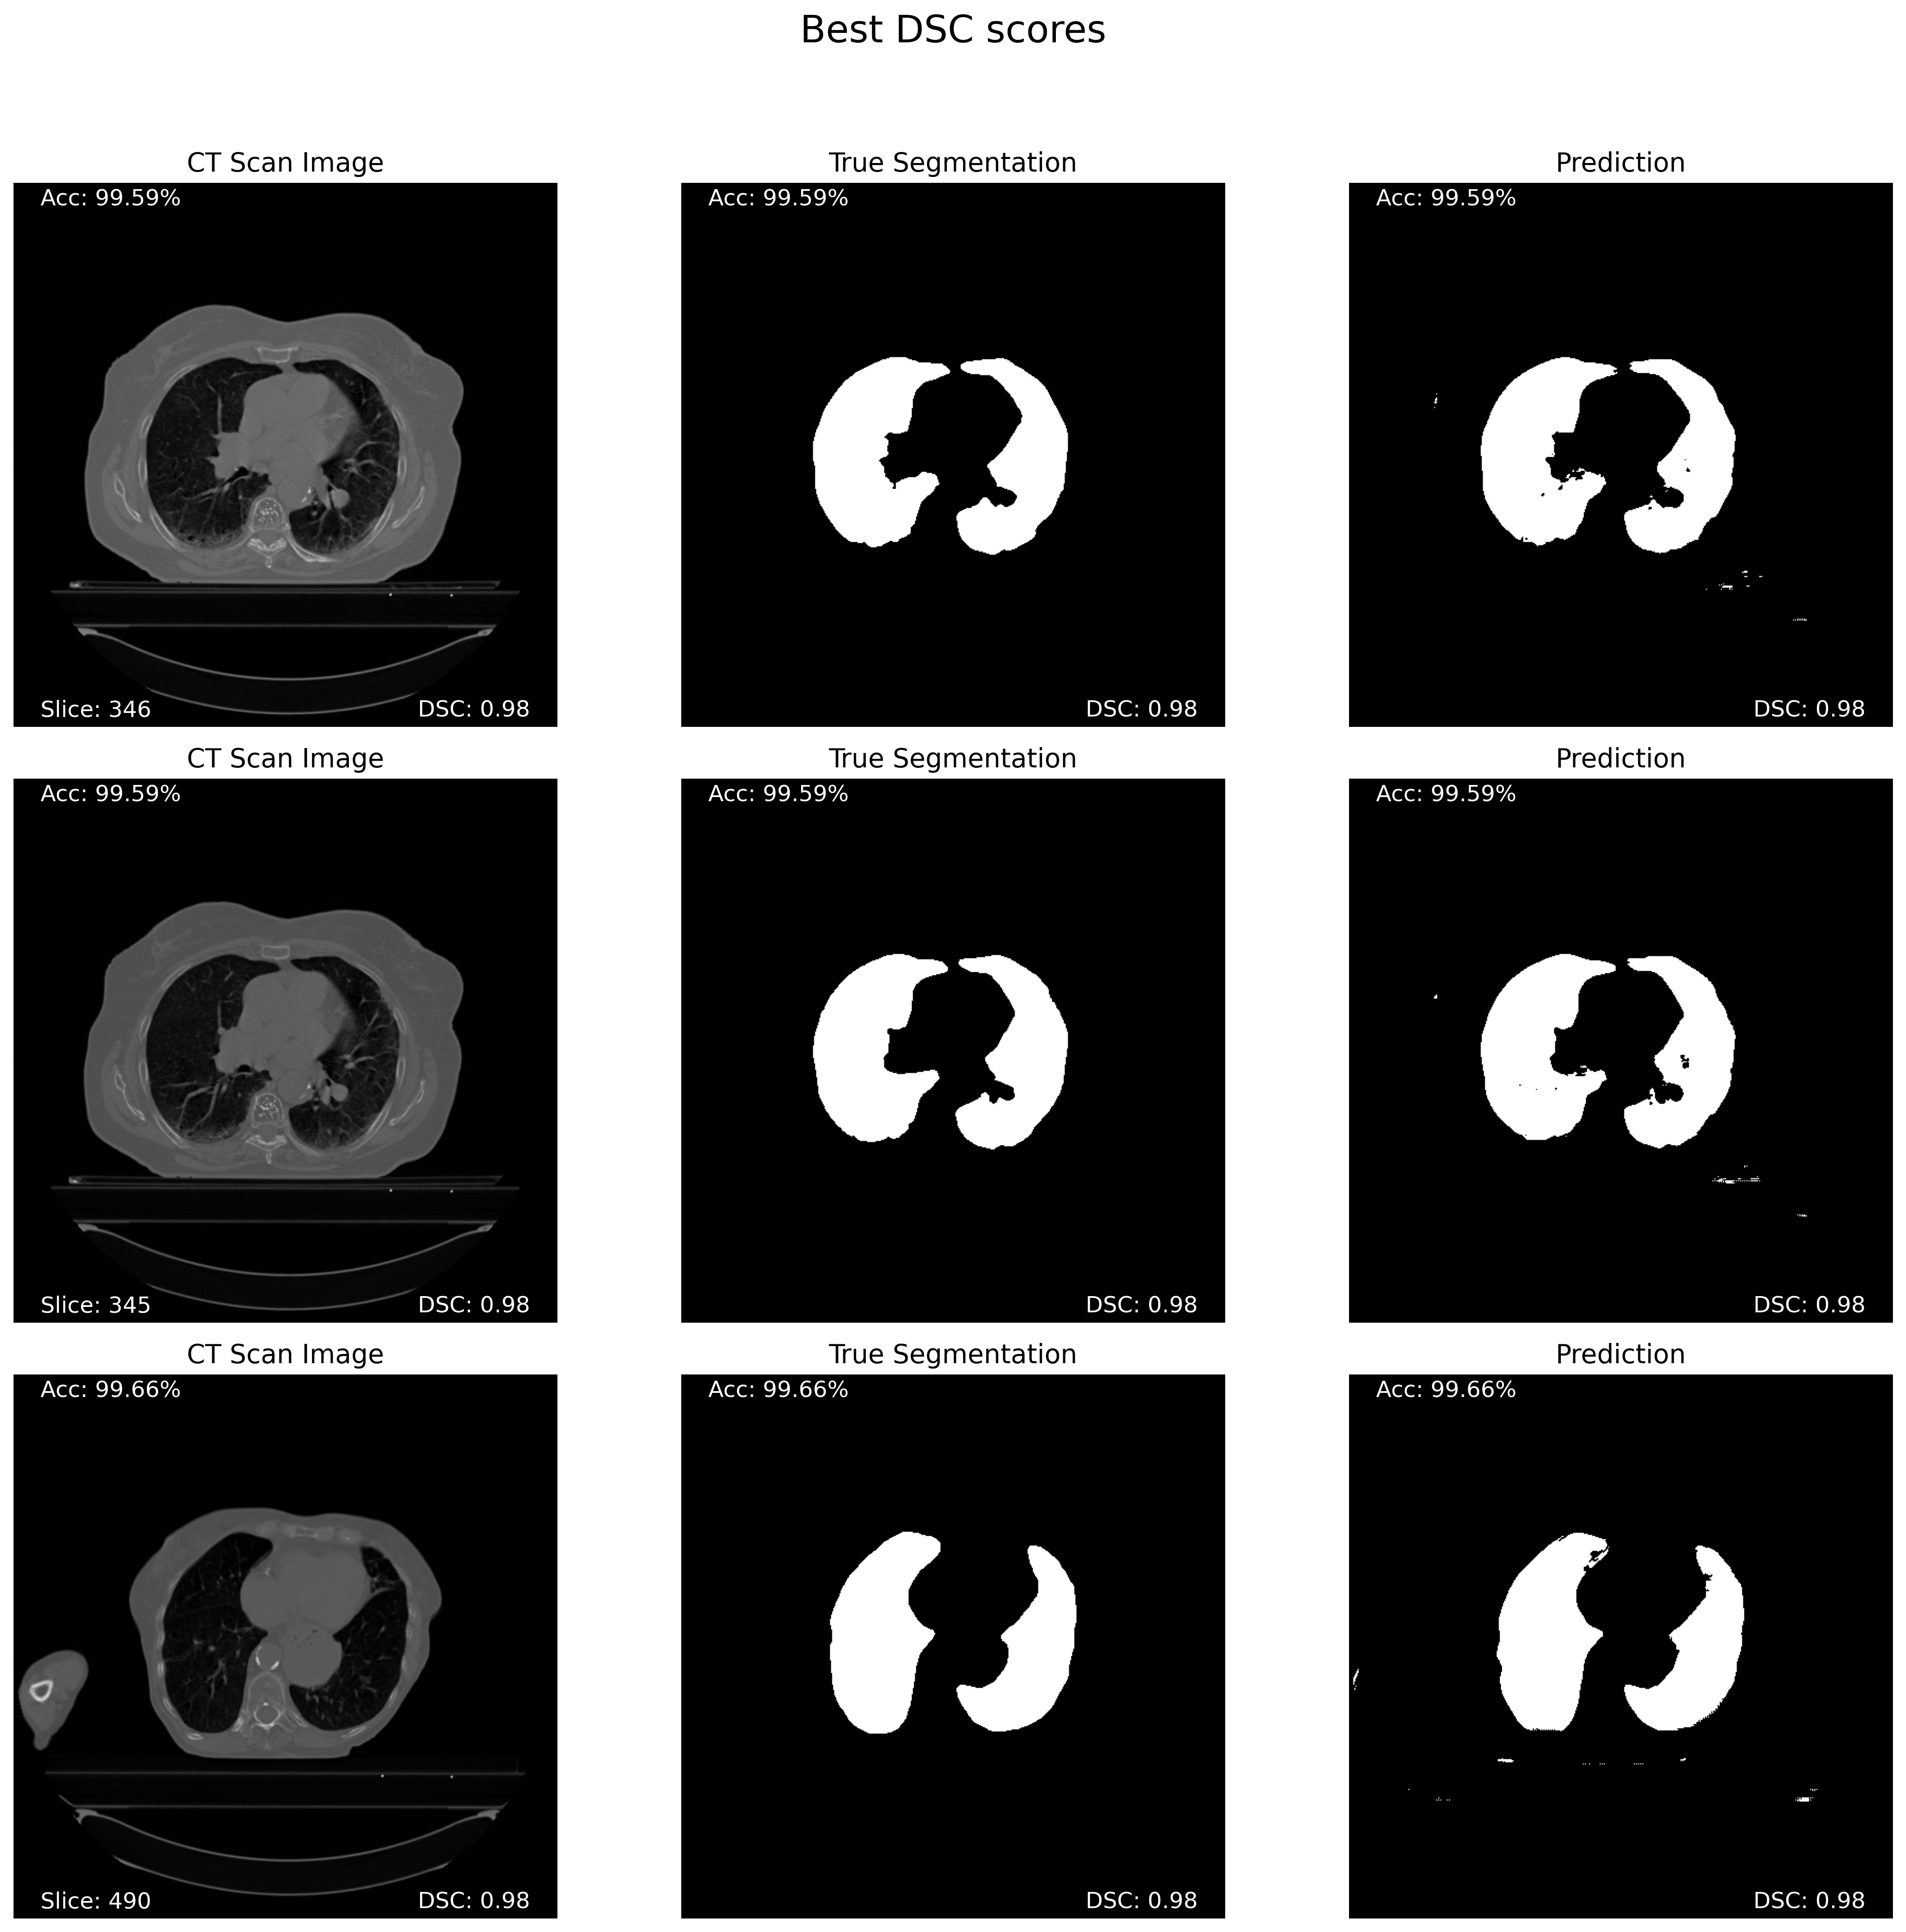
\includegraphics[width=\textwidth]{Best_DSC_scores.png}
    \caption{Axial slices exhibiting the best DSC values}
    \label{fig:best_dsc_scores}
\end{figure}

The slices that display the highest Dice Scores belong to cases 8 and 9, where the model achieves near-perfect accuracies and Dice Scores. Qualitatively, it is evident that the predicted segmentations closely resemble the true segmentations, almost mirroring them identically. This highlights the model's capability to accurately delineate the lungs with high precision.

\begin{figure}[ht]
    \centering
    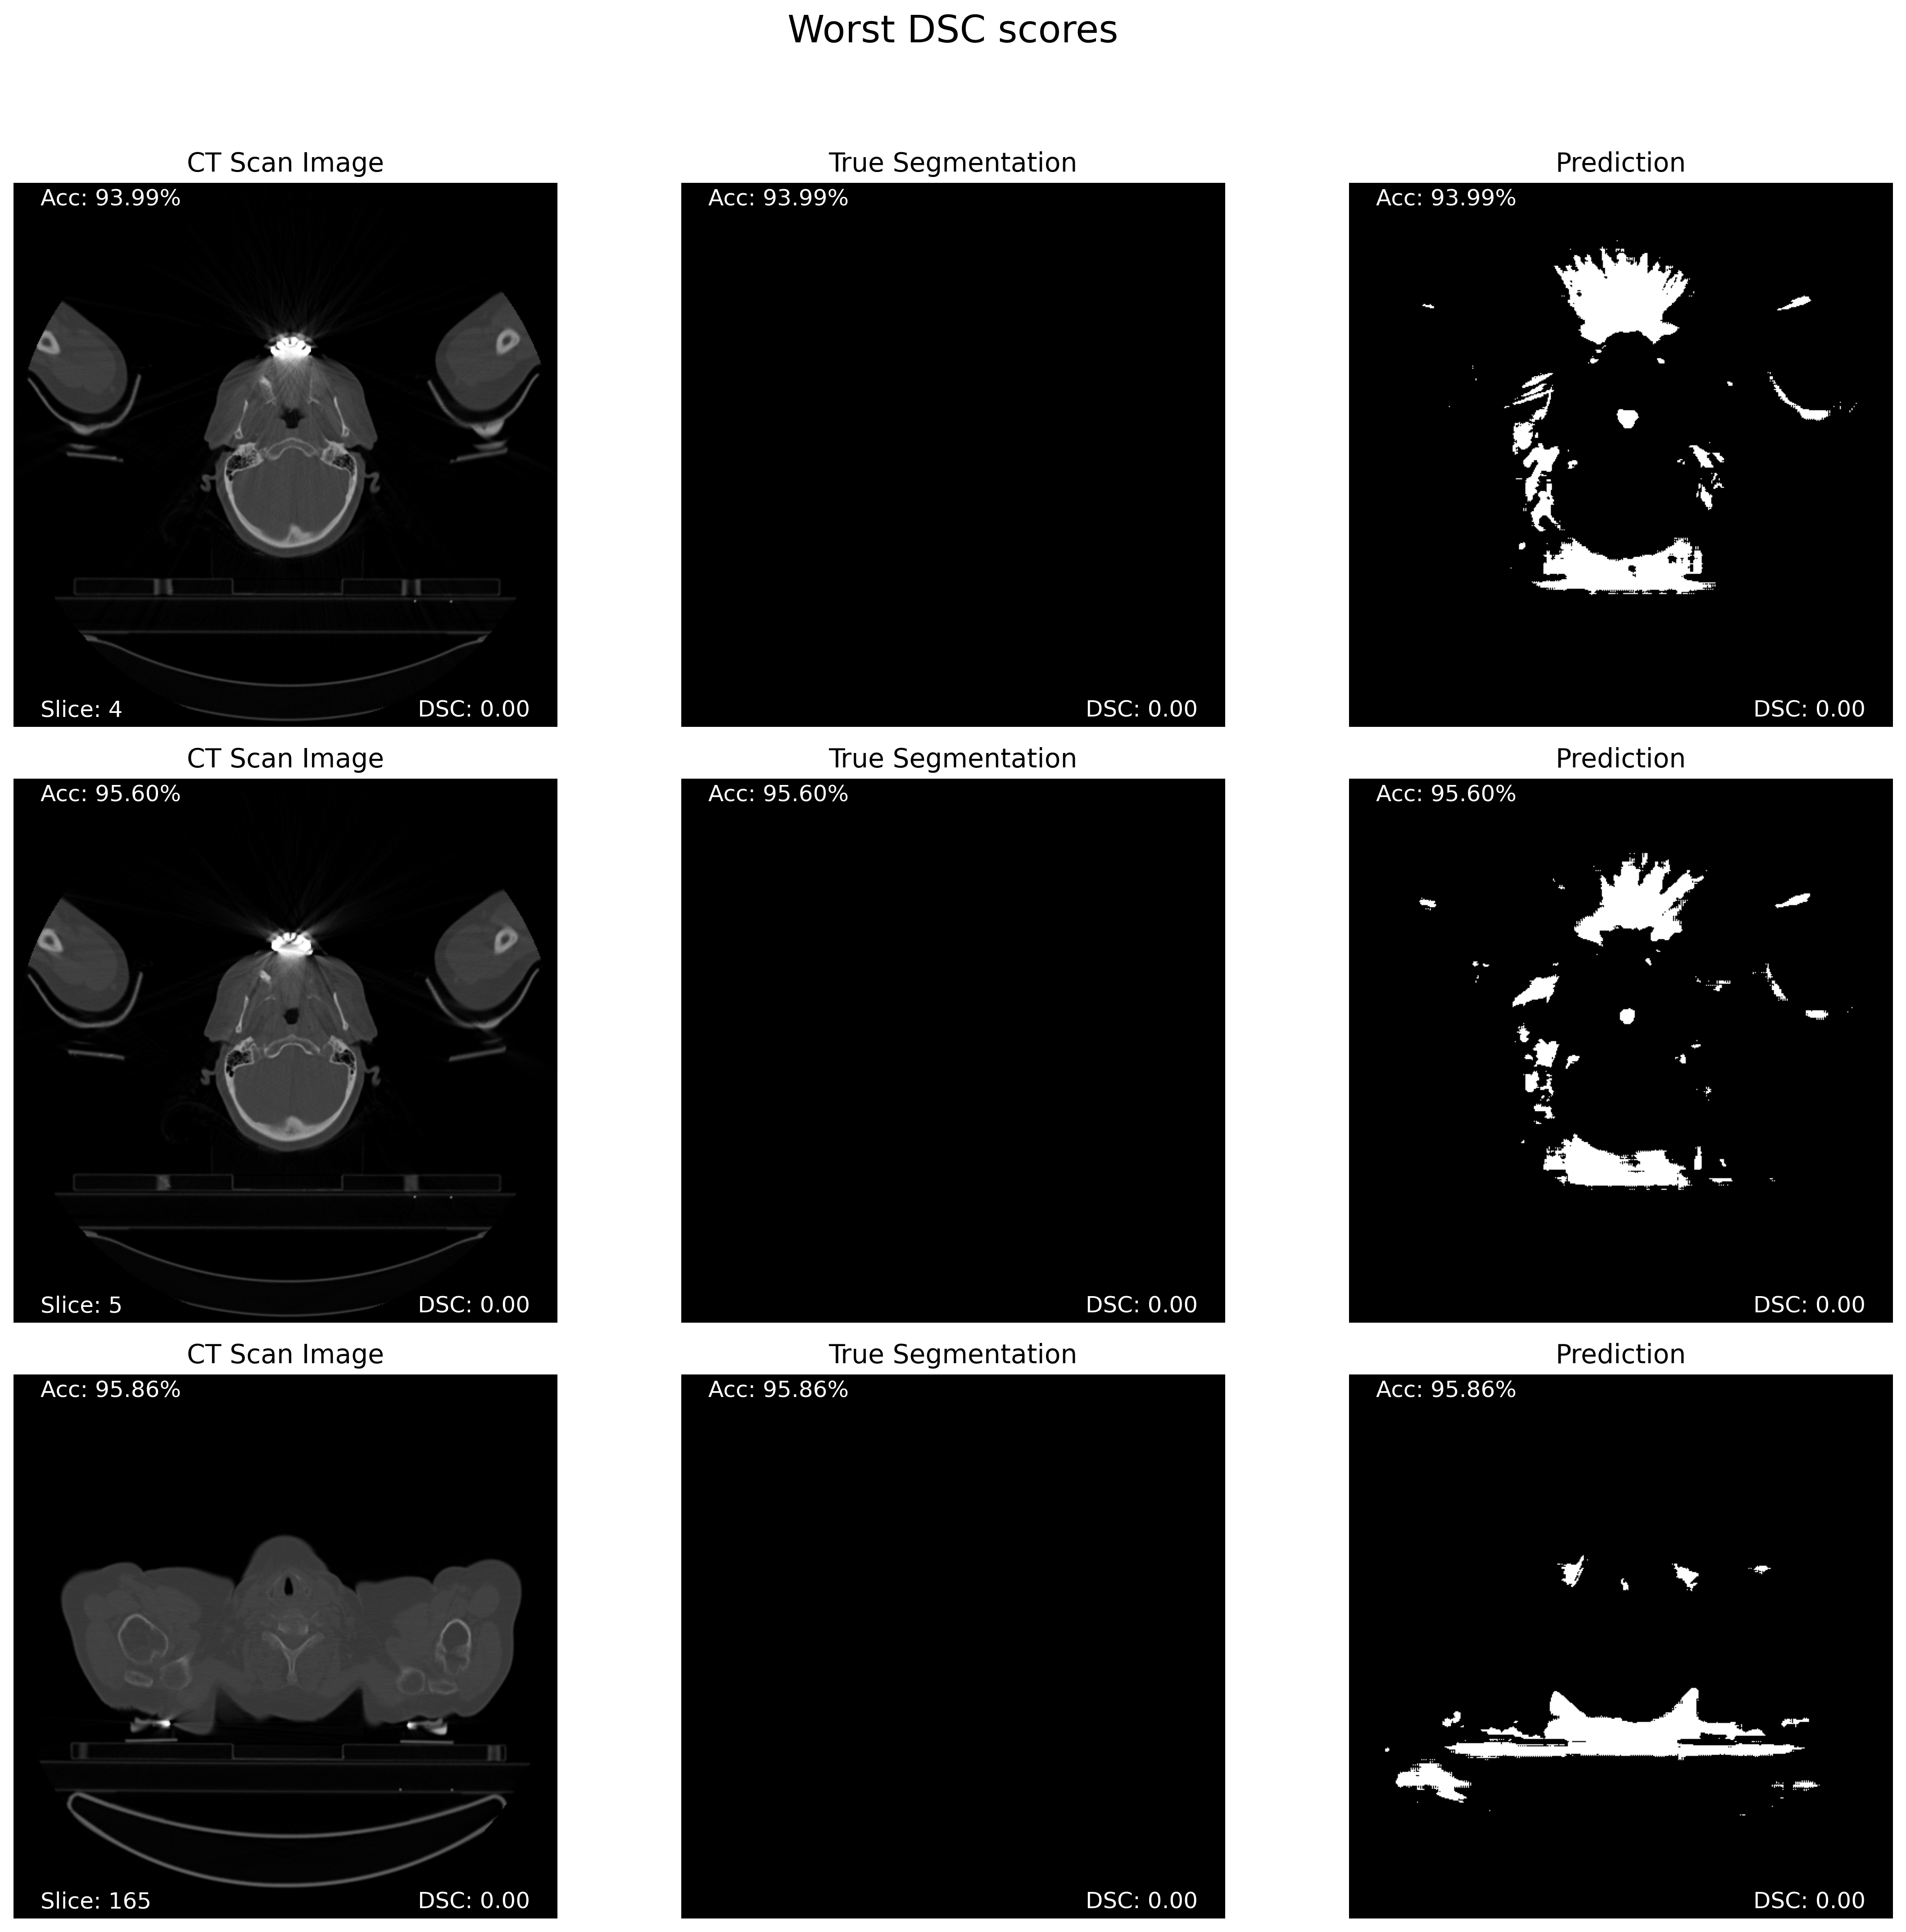
\includegraphics[width=\textwidth]{Worst_DSC_scores.png}
    \caption{Axial slices exhibiting the worst DSC values}
    \label{fig:worst_dsc_scores}
\end{figure}

Figure~\ref{fig:worst_dsc_scores}, which displays the slices that recorded the lowest Dice scores shows CT scans captured before the lungs come into view on the axial plane. This means that the true segmentation is empty and the model should predict an empty segmentation. Contrary to expectations, abstract patterns are predicted by the model resulting in Dice scores of zero. These inaccurately predicted patterns are referred to as ``hallucinations" and have attracted considerable attention due to their uncertain origins in both tomographic image reconstruction and in the field of artificial intelligence (AI) more broadly.\cite{bhadra_hallucinations_2021, noauthor_investigating_nodate, alkaissi_artificial_nodate} Notably, despite the inaccuracies in these specific predictions, the binary accuracy metrics for these slices remain unexpectedly high ($< 93\%$). This discrepancy highlights the limitations of using binary accuracy as a performance metric for the model, and suggests that relying only on this metric may result in poor assessment of model effectiveness.

\begin{figure}[ht]
    \centering
    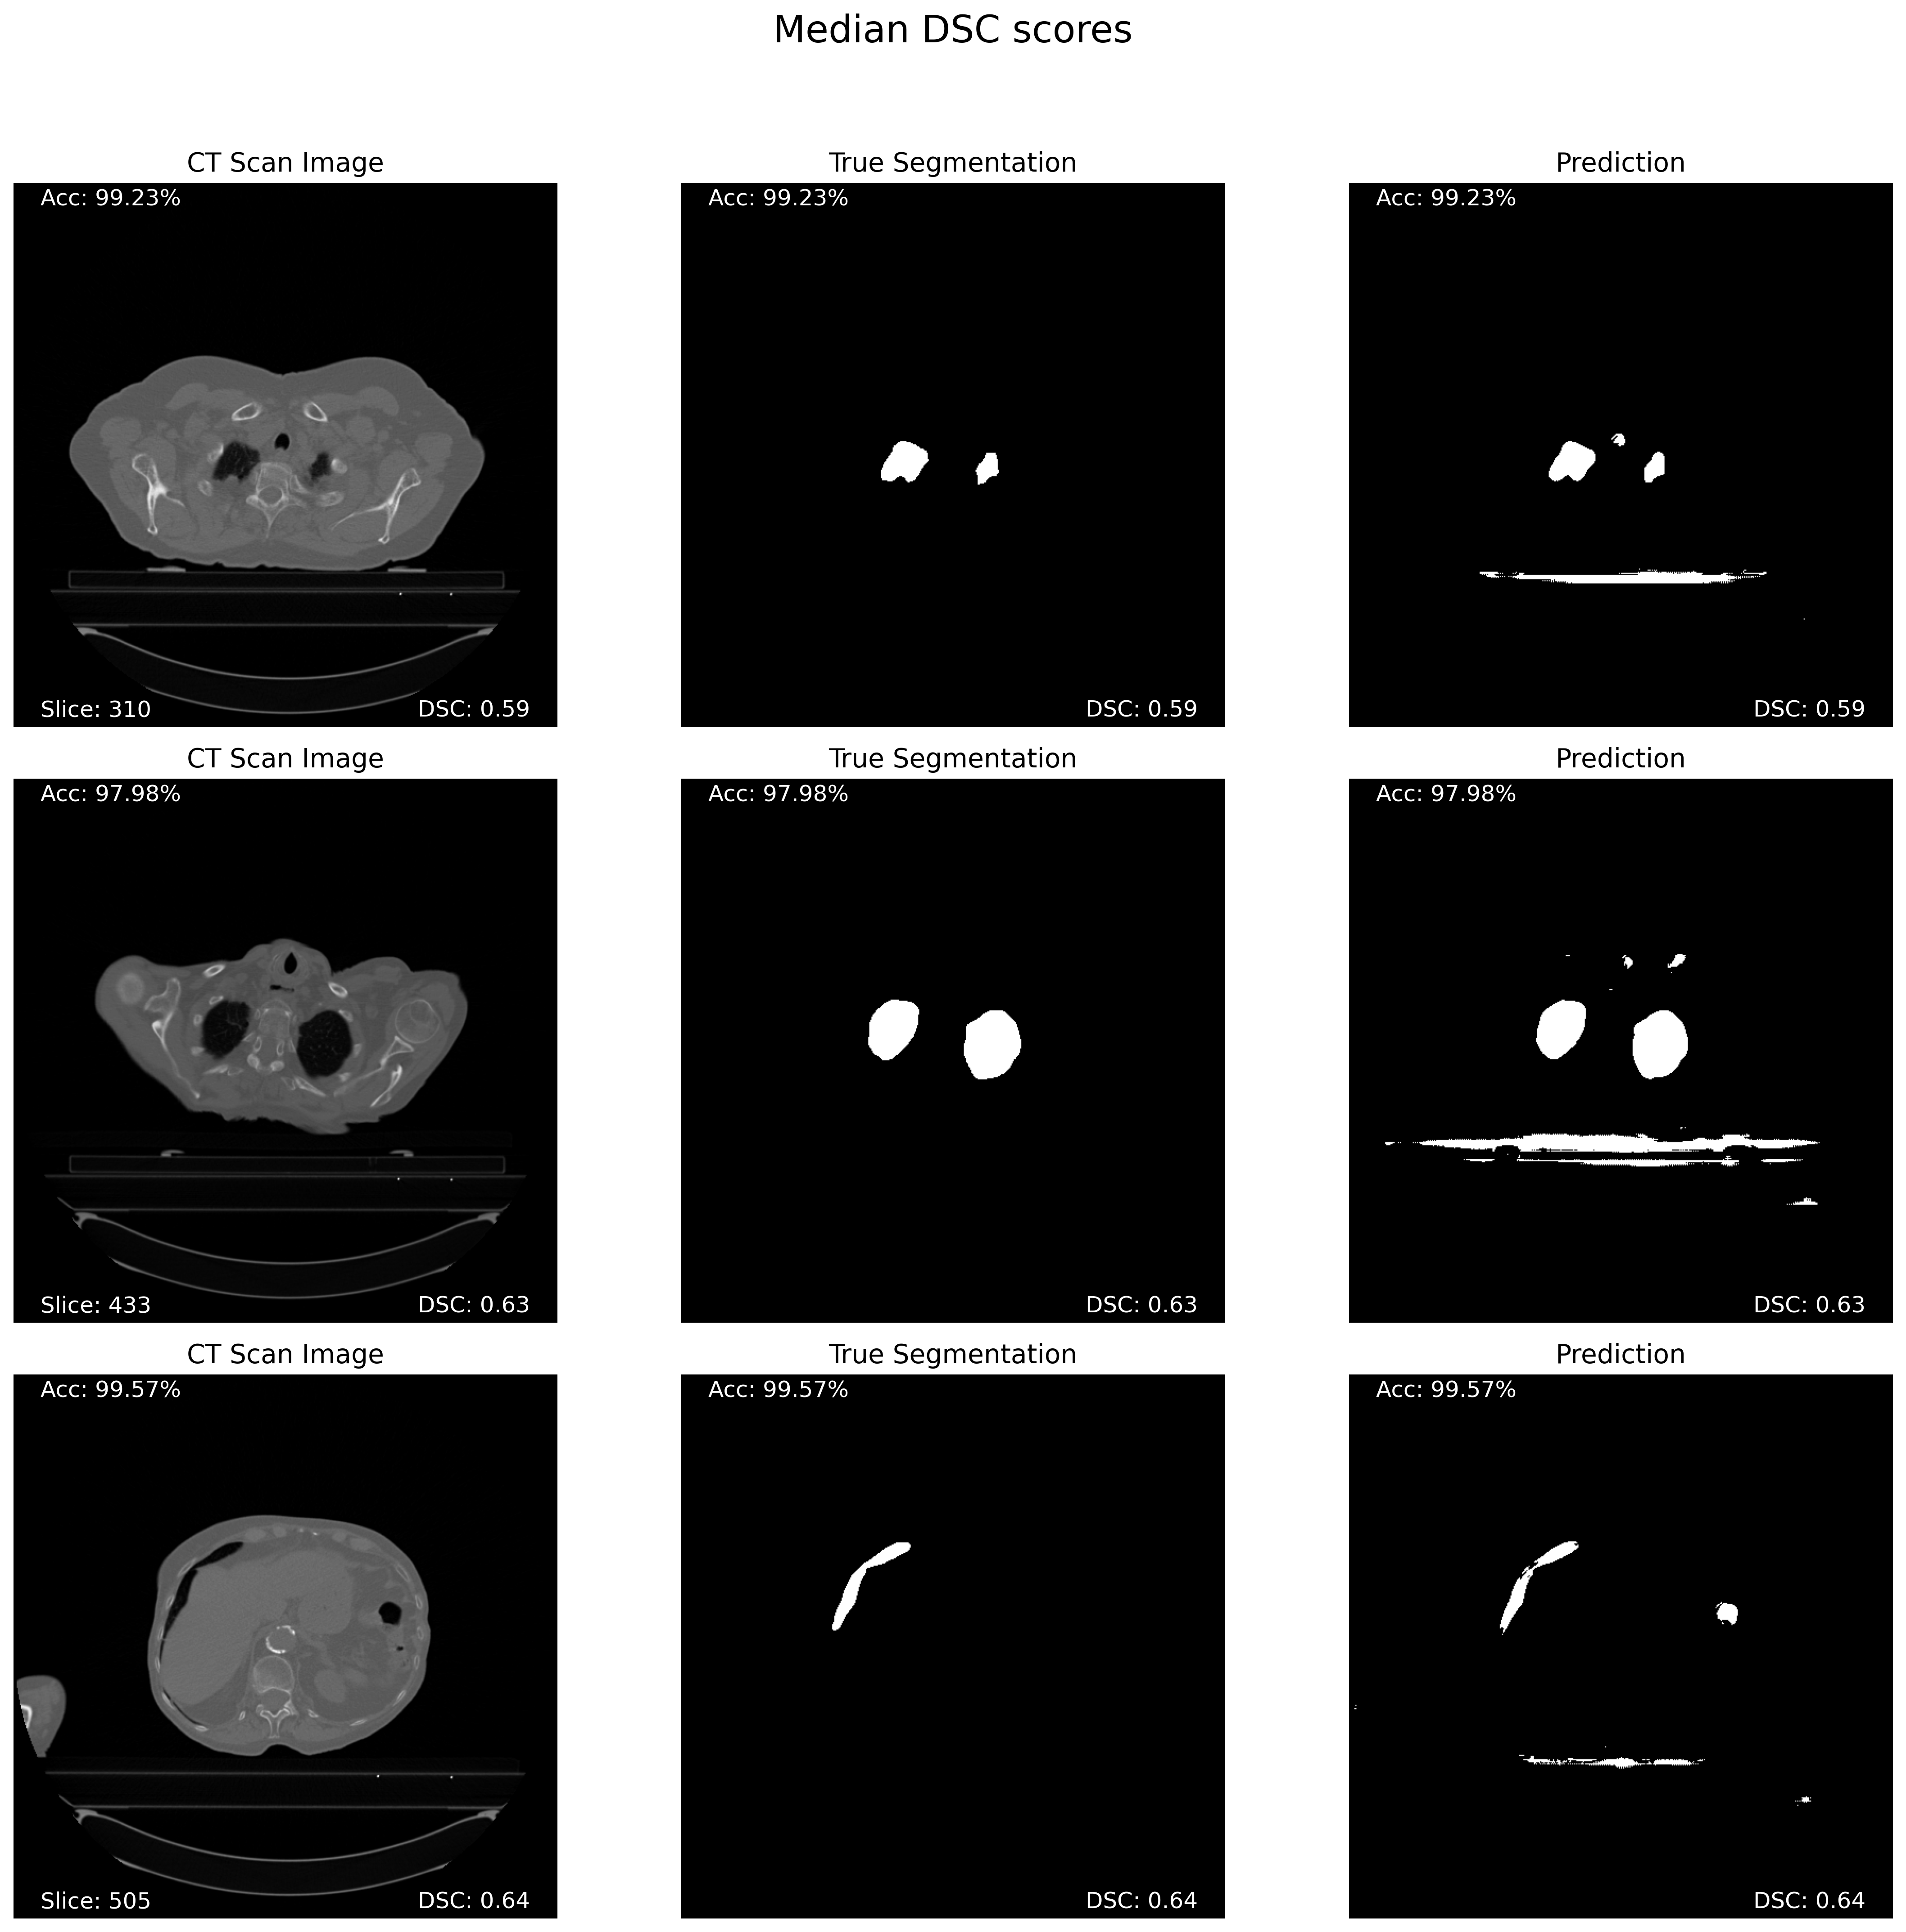
\includegraphics[width=\textwidth]{Median_DSC_scores.png}
    \caption{Axial slices exhibiting median DSC values}
    \label{fig:med_dsc_scores}
\end{figure}

Axial slices achieving median Dice scores are shown in Figure~\ref{fig:med_dsc_scores}. Qualitatively, it can be seen that the model is successful in identifying true segmentations of the lungs in planes where the lung segmentations are particularly small. However, an interesting artifact of the model is the presence of abstract patterns towards the bottom of the predicted segmentations, specifically in regions corresponding to the CT bed. This phenomenon suggests that while the model is generally effective in predicting lung segmentations, it also generates unnecessary or irrelevant patterns in areas devoid of clinical significance.

\chapter{Conclusion}

This project involved the development of a script designed to convert patient DICOM files into 3D NumPy arrays, preparing the data for further analysis. A U-Net model with a lightweight architecture was then trained on these arrays to perform lung segmentation tasks. The training was carried out over 10 epochs with a batch size of 3 and a learning rate of 0.1. The training was carried out twice: first employing a standard binary cross-entropy loss and subsequently adopting a custom loss function that combines binary cross-entropy loss with soft Dice loss. Despite the observation of a higher average loss at the training's conclusion with the custom loss function, the model successfully predicted lung segmentations on a separate test set, as illustrated in Figure~\ref{fig:best_dsc_scores}.

An investigation into the training metrics revealed that the Dice score serves as a more reliable metric for evaluating model performance in the field of image segmentation, compared to simply relying on pixel-level accuracy as measured by binary accuracy. Therefore, an extension of this work would be to investigate the effect of varying the $\alpha$ parameter which controls the ratio of binary cross-entropy loss to soft Dice loss in the custom loss function. It is hypothesised that using more soft Dice loss could lead to better lung segmentations, as minimising this loss helps the model learn the shapes and boundaries of the target segments.

To improve the performance of the U-Net model, three approaches can be employed:

\begin{enumerate}
    \item Reduce learning rate
    \item Augment the training data
    \item Preprocess the training data to remove areas devoid of clinical significance
\end{enumerate}

In this project, the training of both models was conducted with a learning rate of 0.1. Such a learning rate, while facilitating rapid convergence, risks causing the model to overshoot the minima within the loss landscape. Therefore, to enhance model performance, a lower learning rate could be adopted. This adjustment, despite increasing computational demand, aims to ensure a more precise approach to navigating the loss landscape, thereby preventing the oversight of optimal solutions.

Model performance can also be improved through data augmentation: the training set used consisted of 8 cases with 2D 1151 slices. Expanding the training dataset through data augmentations such as rotations, translations, flips, or more advanced techniques such as applying Gaussian blur to the original images\cite{alam_image_2021} can improve the model's robustness and generalization by exposing it to a wider variety of images.

Finally, as discussed in Section~\ref{subsec:dscs}, it was identified that the model incorrectly predicts lung segmentations in regions corresponding to the CT bed. To avoid this, and possibly improve model performance, the training images can be preprocessed to remove sections corresponding to the CT bed, ensuring that the model focuses on learning segmentations within areas of clinical significance.

% References
\printbibliography[heading=bibintoc, title={Bibliography}]

% Appendix
\chapter*{Appendix}
\addcontentsline{toc}{chapter}{Appendix}
\section*{A note on the use of auto-generation tools}
\addcontentsline{toc}{section}{A note on the use of auto-generation tools}

GitHub Copilot was used throughout this project as it is installed on my IDE (Visual Studio Code). Copilot was only used on \inlinecode{.py} and \inlinecode{.ipynb} files (not for writting the \inlinecode{.tex} report) and was limited to to auto-completing lines of code where it made sense to do so (i.e, it was not used to blindly implement functionality, simply to complete code and/or docstring sentences). ChatGPT was used during the coding phase of the project to help with formatting plots (e.g. the GIF in the \inlinecode{README.md} file) and to help accelerate the loading of DICOM files in the first part (by modifying the \inlinecode{load_patient_dicom} function to use concurrency with multithreading). The use of ChatGPT for the report was limited to suggesting alternative wording for sentences which I believed to be too long although direct copy pasting of generated text was avoided.

\end{document}
